%\chapter*{Appendix C}
\textbf{Appendix C}
\chaptermark{Appendix C}

\begin{table}[H]
  \captionsetup{singlelinecheck = false, justification=justified}
\caption{Summary of funding sources}
\label{tab:C_1}
\small
\begin{tabularx}{\textwidth}{@{}ll@{}}
  \toprule
  Acronym & Full name\\
  \midrule
  AVCD & Accelerated Value Chain Development\\
  BMGF & Bill and Melinda Gates Foundation\\
  CCAFS & Climate Change, Agriculture and Food Security\\
  CLiP & Crop-Livestock integration Project\\
  DI & Darwin Initiative\\
  FORETS & FOrmation, Recherche, Environnement dans la TShopo\\
  EU & European Union\\
  LSHTM-IMMANA & The London School of Hygiene \& Tropical Medicine --\\
   & Innovative Metrics and Methods for Agriculture Nutrition Action\\
  SAIRLA & Sustainable Agricultural Intesification Research and Learning in Africa\\
  SIDA & Swedish International Development Agency\\
  USAID & U.S. Agency for International Development\\
\bottomrule
\end{tabularx}
\end{table}

\vspace*{\fill}

%\newpage

\begin{sidewaystable}[ph!]
  \captionsetup{singlelinecheck = false, justification=justified}
  \caption{Summary of household data sources}
  \label{tab:C_2}
  \small
\begin{tabularx}{\textwidth}{
p{\dimexpr 0.26\linewidth-2\tabcolsep}
p{\dimexpr 0.15\linewidth-2\tabcolsep}
p{\dimexpr 0.15\linewidth-2\tabcolsep}
p{\dimexpr 0.21\linewidth-2\tabcolsep}
p{\dimexpr 0.13\linewidth-2\tabcolsep}
p{\dimexpr 0.11\linewidth-2\tabcolsep}}
\toprule
Country (site/region) & Donor & Project & Lead Institute implementing & Year & Number of Households surveyed \\
\midrule
Burkina Faso (country-wide) & SIDA & TreeAID & TreeAID-ILRI & 2018 & 1070 \\
DRC (Yangambi) & EU, CIFOR & FORETS & ICRAF & 2017 & 413 \\
DRC (Kamanyola \& Miti) & IFAD-EU & CLiP & IITA-ILRI & 2017 & 438 \\
Ethiopia (central highlands) & DI & TreeAID & TreeAID-ILRI & 2017 & 707 \\
Ethiopia (Tigray) & DFID & SAIRLA & Bioversity International & 2017 & 253 \\
Kenya (Makueni) & DFID & SAIRLA & Bioversity International & 2017 & 316 \\
Kenya (Nyando) & Maize CRP & CCAFS -- Maize & ILRI & 2016 & 161 \\
Kenya (Baringo \& Kitui) & DFID, LSHTM- IMMANA & SCAN & ICRAF & 2017 & 385 \\
Kenya (Busia, Homa bay, Siaya \& Vihiga) & USAID & AVCD & ILRI & 2017 & 169 \\
Kenya (Wote) & Maize CRP & CCAFS -- Maize & ILRI & 2016 & 160 \\
Malawi (Lilongwe area) & CCAFS & CCAFS & CIMMYT & 2015 & 157 \\
Mali (Diora, Mafoune \& Mandiakuy) & DI & TreeAID & TreeAID-ILRI & 2017 & 363 \\
Tanzania (country-wide) & USAID/BMGF & I4I Galvmed & ILRI & 2017 & 999 \\
Tanzania (incl. Zanzibar) & USDA-FAS & CSA & ICRAF & 2016 & 841 \\
Tanzania (Mtwara \& Lindi) & DFID & SAIRLA & Bioversity International & 2017 & 522 \\
Uganda (Rakai) & CCAFS & CCAFS & Wageningen University & 2017 & 130 \\
Zambia (3 districts) & DFID, LSHTM & SCAN & ICRAF & 2017 & 624 \\
\bottomrule
\end{tabularx}
\end{sidewaystable}

\newpage


\begin{table}[H]
  \captionsetup{singlelinecheck = false, justification=justified}
  \caption{Thresholds for removing observations (removed households may exceed multiple thresholds)}
  \label{tab:C_3}
  \small
\begin{tabularx}{\textwidth}{@{}lYY@{}}
  %{
%p{\dimexpr 0.48\linewidth-2\tabcolsep}
%p{\dimexpr 0.22\linewidth-2\tabcolsep}
%p{\dimexpr 0.29\linewidth-2\tabcolsep}}
\toprule
Variable & Threshold & Number of observations \\
\midrule
Household members (adult equivalents) & {\textgreater} 30 & 48 \\
 & = 0 & 68 \\
Land area (ha) & {\textgreater} 100 & 9 \\
Livestock holdings (TLUs) & {\textgreater} 250 & 72 \\
Income (PPP) & {\textgreater}100,000 & 93 \\
Modified Household Diet Diversity & = 0 & 776 \\
Enumerator assessed reliability & Regular doubts & 25 \\
 & Occasional doubts & 200 \\
Enumerator assessed ease to build rapport & Very difficult & 26 \\
\bottomrule
\end{tabularx}
\end{table}

%\smallskip
%\vspace{1cm}

Observations were removed in instances where no MHDD was enumerated or where land cultivated, livestock holdings or household population were non-credible (n = 1,355). Approximately 10\% of observations were removed from Burkina Faso, Kenya and Tanzania. After removing these observations, 6,612 households remained in this study.


\newpage

\begin{table}[H]
  \captionsetup{singlelinecheck = false, justification=justified}
  \caption{Sources of micronutrients in Modified Household Diet Diversity categories in East Africa (source defined as providing 15\% of adult male requirement)}
  \label{tab:C_4}
  \small
\begin{tabularx}{\textwidth}{@{}lYYYYYYYYYYY@{}}
%  {
%p{\dimexpr 0.19\linewidth-2\tabcolsep}
%p{\dimexpr 0.05\linewidth-2\tabcolsep}
%p{\dimexpr 0.04\linewidth-2\tabcolsep}
%p{\dimexpr 0.06\linewidth-2\tabcolsep}
%p{\dimexpr 0.07\linewidth-2\tabcolsep}
%p{\dimexpr 0.09\linewidth-2\tabcolsep}
%p{\dimexpr 0.09\linewidth-2\tabcolsep}
%p{\dimexpr 0.08\linewidth-2\tabcolsep}
%p{\dimexpr 0.08\linewidth-2\tabcolsep}
%p{\dimexpr 0.08\linewidth-2\tabcolsep}
%p{\dimexpr 0.09\linewidth-2\tabcolsep}
%p{\dimexpr 0.07\linewidth-2\tabcolsep}}
\toprule
~ & Ca${\dag}$ & Fe & Zn & VitA & Thiamine & Riboflavin & Niacin & Vitamin B6 & Folate & Vitamin B12 & Vitamin C \\
\midrule
Grains, roots, tubers and plantain & & x & & & x & & x & x & & & \\
Pulses & & & & & & & & x & x & & \\
Nuts and seeds & x & x & x & & x & x & x & x & x & & \\
Dairy & x & & & & & & & & & x & \\
Meat, poultry and fish & & & x & x & & x & x & x & & x & \\
Eggs & & & & x & & x & & & & x & \\
Leafy vegetables & & & & x & & & & & & & x \\
Vitamin A rich vegetables & & x & x & x & x & & & & & & x \\
Other vegetables & & & & & & & & & & & \\
Other fruits & & & & & & & & & & & x \\
\bottomrule
\end{tabularx}
\footnotesize
\raggedright
$^{\dag}$Threshold set at 12\%
\end{table}



\begin{table}[H]
  \small
  \raggedright Table \ref{tab:C_4} continued
\begin{tabularx}{\textwidth}%{@{}lYYYYYYYY@{}}
  {
p{\dimexpr 0.26\linewidth-2\tabcolsep}
p{\dimexpr 0.06\linewidth-2\tabcolsep}
p{\dimexpr 0.07\linewidth-2\tabcolsep}
p{\dimexpr 0.07\linewidth-2\tabcolsep}
p{\dimexpr 0.07\linewidth-2\tabcolsep}
p{\dimexpr 0.1\linewidth-2\tabcolsep}
p{\dimexpr 0.14\linewidth-2\tabcolsep}
p{\dimexpr 0.12\linewidth-2\tabcolsep}
p{\dimexpr 0.1\linewidth-2\tabcolsep}}
\toprule
~ & Cu & K & Mg & Mn & P & Pantothenic acid & Vitamin D & Vitamin E \\
\midrule
Grains, roots, tubers and plantain & & & x & x & x & & & \\
Pulses & & & & & & & & \\
Nuts and seeds & x & x & x & x & x & x & & x \\
Dairy & & & & & x & & & \\
Meat, poultry and fish & & & & & x & & & \\
Eggs & & & & & x & x & x & \\
Leafy vegetables & & & & & & & & \\
Vitamin A rich fruits and vegetables & x & & x & x & x & & & x \\
Other vegetables & & & & & & & & \\
Other fruits & & & & & & & & \\
\bottomrule
\end{tabularx}
\end{table}




\begin{table}[H]
  \captionsetup{singlelinecheck = false, justification=justified}
  \caption{Sources of micronutrients in Modified Household Diet Diversity categories in Central and West Africa (source defined as providing 15\% of adult male requirement)}
  \label{tab:C_5}
  \small
\begin{tabularx}{\textwidth}%{@{}lYYYYYYYYYYY@{}}
  {
p{\dimexpr 0.19\linewidth-2\tabcolsep}
p{\dimexpr 0.05\linewidth-2\tabcolsep}
p{\dimexpr 0.04\linewidth-2\tabcolsep}
p{\dimexpr 0.06\linewidth-2\tabcolsep}
p{\dimexpr 0.07\linewidth-2\tabcolsep}
p{\dimexpr 0.09\linewidth-2\tabcolsep}
p{\dimexpr 0.09\linewidth-2\tabcolsep}
p{\dimexpr 0.08\linewidth-2\tabcolsep}
p{\dimexpr 0.08\linewidth-2\tabcolsep}
p{\dimexpr 0.08\linewidth-2\tabcolsep}
p{\dimexpr 0.09\linewidth-2\tabcolsep}
p{\dimexpr 0.07\linewidth-2\tabcolsep}}
\toprule
~ & Ca${\dag}$ & Fe & Zn & VitA & Thiamine & Riboflavin & Niacin & Vitamin B6 & Folate & Vitamin B12 & Vitamin C \\
\midrule
Grains, roots, tubers and plantain & & x & & & x & & & x & & & \\
Pulses & & x & x & & x & x & & x & x & & \\
Nuts and seeds & x & x & x & & x & & x & x & x & & \\
Dairy & x & & & & & x & & & & x & \\
Meat, poultry and fish & & x & x & x & x & x & x & x & & x & \\
Eggs & & & & x & & x & & & & x & \\
Leafy vegetables & & & & x & & & & & x & & x \\
Vitamin A rich vegetables & & x & & & x & & & & & & x \\
Other vegetables & & & & & & & & & & & x \\
Other fruits & & & & & & & & & & & x \\
\bottomrule
\end{tabularx}
\footnotesize
\raggedright
$^{\dag}$Threshold set at 12\%
\end{table}

\begin{table}[H]
  \small
  \raggedright Table \ref{tab:C_5} continued
\begin{tabularx}{\textwidth}%{@{}lYYYYYYYY@{}}
  {
p{\dimexpr 0.26\linewidth-2\tabcolsep}
p{\dimexpr 0.06\linewidth-2\tabcolsep}
p{\dimexpr 0.07\linewidth-2\tabcolsep}
p{\dimexpr 0.07\linewidth-2\tabcolsep}
p{\dimexpr 0.07\linewidth-2\tabcolsep}
p{\dimexpr 0.1\linewidth-2\tabcolsep}
p{\dimexpr 0.14\linewidth-2\tabcolsep}
p{\dimexpr 0.12\linewidth-2\tabcolsep}
p{\dimexpr 0.1\linewidth-2\tabcolsep}}
\toprule
~ & Cu & K & Mg & Mn & P & Pantothenic acid & Vitamin D & Vitamin E \\
\midrule
Grains, roots, tubers and plantain & & & x & x & x & & & \\
Pulses & x & x & x & x & x & x & & \\
Nuts and seeds & x & x & x & x & x & x & & x \\
Dairy & & & & & x & & & \\
Meat, poultry and fish & & & & & x & x & x & \\
Eggs & & & & & x & x & x & \\
Leafy vegetables & & & & & & & & x \\
Vitamin A rich fruits and vegetables & & & x & x & & & & \\
Other vegetables & & & & & & & & \\
Other fruits & & & & & & & & \\
\bottomrule
\end{tabularx}
\end{table}

\vspace*{\fill}



%\newpage

%\vspace*{\fill}

The quantified adequacy ratios among subsistence households (n = 264) varied substantially by nutrient (\ref{fig:A_1} and \ref{fig:A_2}). There were consistently large gaps in the availability of vitamin A and vitamin C. Conversely, there were no micronutrient requirements that were consistently sufficient for all subsistence households.

\begin{figure}[H]
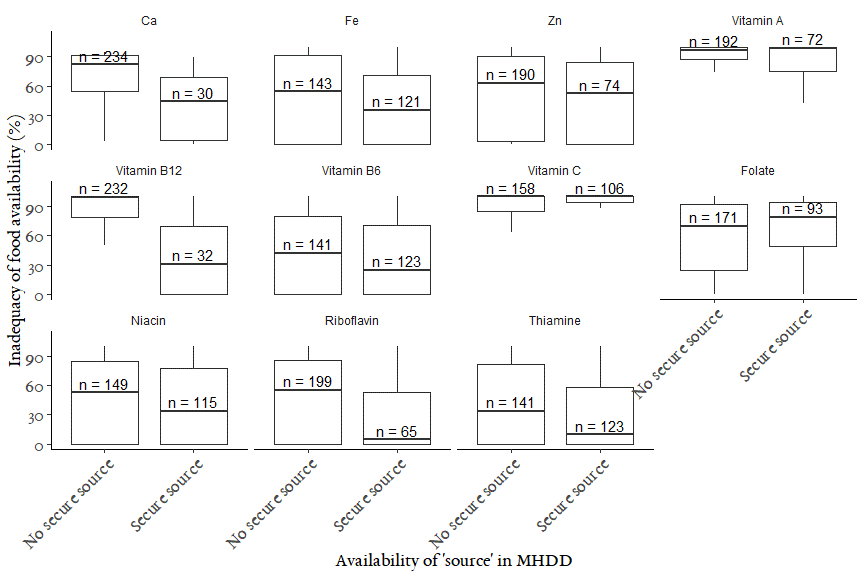
\includegraphics[width=1\textwidth]{Appendix/Ch6_1.png}
  \captionsetup{singlelinecheck = false, justification=justified} %left justify caption
  \caption{Comparison of all micronutrient gaps from farm production (y axis) and `sources' in the Modified Household Diet Diversity (MHDD) indicator (x axis). This figure is limited to farm dependent households. The `n' above the median line is the number of farm dependent households. A `secure source' is defined by a household consuming a food category on a daily basis in both the flush and lean period. The number of observations are indicated on the figure}
  \label{fig:A_1}
\end{figure}

\begin{figure}[H]
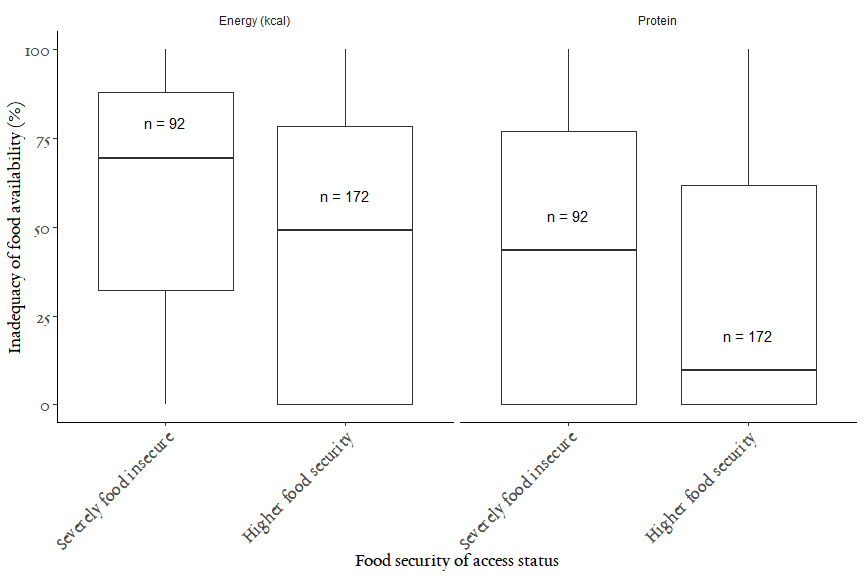
\includegraphics[width=1\textwidth]{Appendix/Ch6_2.png}
  \captionsetup{singlelinecheck = false, justification=justified} %left justify caption
  \caption{Comparison of dietary gaps from farm production and Household Food Insecurity of Access Prevalence (MHFIAP) indicator. This figure is limited to farm dependent households. Food security status is represented by two categories: `Severely food insecure' and an amalgamation of the higher 3 MHFIAP food security categories into the category `Higher food security'. The number of observations are indicated on the figure}
  \label{fig:A_2}
\end{figure}


\vspace*{\fill}
%\newpage

\begin{sidewaystable}[ph!]
  \captionsetup{singlelinecheck = false, justification=justified}
  \caption{Associations between nutrition (dependent variables in columns) and livelihood characteristics and agroecological zone (AEZ). Logistic\textasciicircum{} and negative binomial$^{\dag}$ regressions, displaying the direction of association for statistically significant explanatory variables (n = 6,353)}
  \label{tab:C_7}
  \small
%\begin{tabular}{L{4cm} C{1.5cm} C{1.5cm} C{1.5cm} C{1cm} C{1cm} C{1cm} C{1cm} C{1.5cm} C{1.5cm} C{1.5cm} }
%16.5
\begin{tabularx}{\textwidth}{
p{\dimexpr 0.20\linewidth-2\tabcolsep}
p{\dimexpr 0.08\linewidth-2\tabcolsep}
p{\dimexpr 0.08\linewidth-2\tabcolsep}
p{\dimexpr 0.08\linewidth-2\tabcolsep}
p{\dimexpr 0.08\linewidth-2\tabcolsep}
p{\dimexpr 0.08\linewidth-2\tabcolsep}
p{\dimexpr 0.08\linewidth-2\tabcolsep}
p{\dimexpr 0.08\linewidth-2\tabcolsep}
p{\dimexpr 0.08\linewidth-2\tabcolsep}
p{\dimexpr 0.08\linewidth-2\tabcolsep}
p{\dimexpr 0.08\linewidth-2\tabcolsep}}
\toprule
 & MHFIAP\textasciicircum{} & HDD flush period$^{\dag}$ & HDD lean period$^{\dag}$ & Ca\textasciicircum{} & Fe\textasciicircum{} & Thiamine\textasciicircum{} & Riboflavin\textasciicircum{} & Niacin\textasciicircum{} & Vitamin B6\textasciicircum{} & Vitamin B12\textasciicircum{} \\
\midrule
Intercept & 0.73 (1.15) & 1.17 (0.15)* & 0.41 (0.2) & -2.39 (0.99) & 0.15 (0.67) & 0.18 (0.63) & -0.14 (0.75) & -0.11 (0.86) & 0.42 (0.66) & -2.05 (0.86)* \\
Household inhabitants (adulteq.) & 0.08 (0.04) & 0.02 (0.01)* & 0.04 (0.01)* & 0.08 (0.06)* & 0.02 (0.05) & 0.03 (0.05) & -0.05 (0.06) & 0.01 (0.06) & -0.01 (0.05) & 0.14 (0.06)* \\
Female household head (yes) & -0.23 (0.1)* & -0.01 (0.02) & 0 (0.02) & -0.39 (0.12) & 0.08 (0.11) & 0.07 (0.11) & -0.09 (0.11) & 0.02 (0.11) & 0.15 (0.11) & -0.09 (0.11) \\
Children under 10 (yes) & -0.63 (0.1)* & 0.01 (0.02) & -0.05 (0.02)* & -0.3 (0.11) & 0.01 (0.11) & 0.01 (0.11) & 0.02 (0.1) & -0.05 (0.11) & -0.07 (0.11) & -0.12 (0.11) \\
\arrayrulecolor{black!30}\midrule
Land cultivated (ha) & -0.01 (0.03) & 0 (0.01) & 0 (0.01) & 0.23 (0.09)* & 0.13 (0.06)* & 0.13 (0.06)* & 0.03 (0.08) & 0.11 (0.06) & 0.15 (0.07)* & 0.1 (0.08) \\
Livestock holdings (TLU) & -0.1 (0.03)* & 0.04 (0.02)* & -0.01 (0.01)* & 0.12 (0.05)* & 0.41 (0.13)* & 0.15 (0.05)* & 0.38 (0.12)* & 0.41 (0.14)* & 0.25 (0.06)* & 0.18 (0.05)* \\
Market participation (\% kcal sold) & 0.65 (0.15)* & 0.11 (0.03)* & 0.21 (0.04)* & 0.84 (0.18)* & 0.27 (0.15) & 0.31 (0.15)* & 0.37 (0.16)* & 0.04 (0.16) & 0.31 (0.16)* & 0.75 (0.17)* \\
Off-farm income (yes) & 0.2 (0.09)* & 0.05 (0.02)* & 0.08 (0.02)* & 0.13 (0.1)* & 0.37 (0.09)* & 0.37 (0.09)* & 0.34 (0.09)* & 0.47 (0.1)* & 0.41 (0.09)* & 0.4 (0.1)* \\
Gross income (PPP) & 0.41 (0.06)* & 0.03 (0.01)* & 0.05 (0.01)* & 0.17 (0.05)* & 0.06 (0.04) & 0.06 (0.04) & 0.15 (0.05)* & 0.08 (0.05) & 0.08 (0.05) & 0.16 (0.05)* \\
\arrayrulecolor{black}\bottomrule
%\end{tabular}
\end{tabularx}
\end{sidewaystable}

\vspace*{\fill}



\begin{sidewaystable}[ph!]
\small
\raggedright Table \ref{tab:C_7} continued
\label{tab:C_7_1}

\begin{tabularx}{\textwidth}{
p{\dimexpr 0.20\linewidth-2\tabcolsep}
p{\dimexpr 0.08\linewidth-2\tabcolsep}
p{\dimexpr 0.08\linewidth-2\tabcolsep}
p{\dimexpr 0.08\linewidth-2\tabcolsep}
p{\dimexpr 0.08\linewidth-2\tabcolsep}
p{\dimexpr 0.08\linewidth-2\tabcolsep}
p{\dimexpr 0.08\linewidth-2\tabcolsep}
p{\dimexpr 0.08\linewidth-2\tabcolsep}
p{\dimexpr 0.08\linewidth-2\tabcolsep}
p{\dimexpr 0.08\linewidth-2\tabcolsep}
p{\dimexpr 0.08\linewidth-2\tabcolsep}}
\toprule
 & MHFIAP\textasciicircum{} & HDD flush period$^{\dag}$ & HDD lean period$^{\dag}$ & Ca\textasciicircum{} & Fe\textasciicircum{} & Thiamine\textasciicircum{} & Riboflavin\textasciicircum{} & Niacin\textasciicircum{} & Vitamin B6\textasciicircum{} & Vitamin B12\textasciicircum{} \\
 \midrule
Crop production diversity${\ddag}$ & 0.1 (0.04)* & 0.01 (0.01) & 0.03 (0.01)* & -0.08 (0.04) & 0.1 (0.04)* & 0.1 (0.04)* & -0.01 (0.04) & 0.14 (0.04)* & 0.07 (0.04) & -0.07 (0.04) \\
Livestock product diversity${\ddag}$ & 0.32 (0.05)* & 0.05 (0.01)* & 0.05 (0.01)* & 0.79 (0.06)* & -0.15 (0.05)* & -0.13 (0.05)* & -0.05 (0.05) & -0.07 (0.06) & -0.1 (0.05)* & 0.68 (0.05)* \\
AEZ (sub-)humid{\S} & 0.4 (0.16)* & 0.05 (0.02)* & 0.07 (0.05) & 0.88 (0.2)* & -0.37 (0.18)* & -0.45 (0.18)* & 0.42 (0.19)* & -0.31 (0.2) & -0.48 (0.18)* & 0.76 (0.19)* \\
Household members:AEZ{\S} & NS & NS & 0.02 (0.02) & NS & 0.03 (0.07) & NS & 0.17 (0.08)* & NS & NS & NS \\
Land cultivated:AEZ{\S} & NS & NS & NS & 0.21 (0.12)* & NS & NS & -0.17 (0.11) & 0.28 (0.19) & NS & 0.15 (0.11) \\
Livestock holdings:AEZ{\S} & NS & 0.09 (0.03)* & NS & NS & 0.4 (0.18)* & NS & 0.19 (0.16) & NS & NS & NS \\
Market participation:AEZ{\S} & -1.54 (0.22)* & NS & 0.07 (0.05) & -0.55 (0.24) & NS & NS & NS & NS & NS & -0.45 (0.23)* \\
Crop production diversity:AEZ{\S} & NS & NS & 0.05 (0.01)* & NS & 0.27 (0.05)* & 0.27 (0.05)* & 0.06 (0.05) & 0.28 (0.06)* & 0.26 (0.05)* & NS \\
\arrayrulecolor{black}\bottomrule
\end{tabularx}
\footnotesize
\raggedright
\textasciicircum{} Logistic regression
$^{\dag}$ negative binomial regression
$^{\ddag}$ Number of crop/livestock MHDD categories produced
$^{\S}$ AEZ reference category = semi-arid
\end{sidewaystable}


\begin{figure}[H]
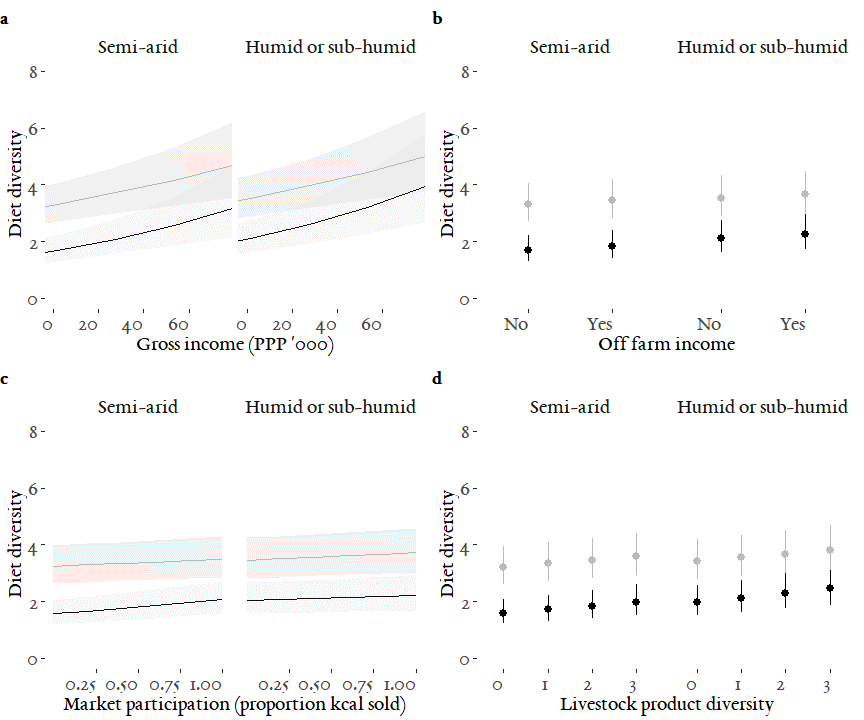
\includegraphics[width=1\textwidth]{Appendix/Ch6_3.png}
    \captionsetup{singlelinecheck = false, justification=justified} %left justify caption
  \caption{Predicted association between other variables and MHDD in the the flush (grey line/point) and lean (black line/point) periods by agroecological zone}
  \label{fig:A_3}
\end{figure}



\begin{table}[H]
  \captionsetup{singlelinecheck = false, justification=justified}
  \caption{Proportion of households in farm types by region}
  \label{tab:C_8}
  \small
\begin{tabularx}{\textwidth}{@{}lYYY@{}}
%  {
%p{\dimexpr 0.35\linewidth-2\tabcolsep}
%p{\dimexpr 0.18\linewidth-2\tabcolsep}
%p{\dimexpr 0.23\linewidth-2\tabcolsep}
%p{\dimexpr 0.23\linewidth-2\tabcolsep}}
\toprule
Farm type~ & East Africa & Central Africa & West Africa \\
\midrule
Specialised cropping & 0.69 & 0.12 & 0.19 \\
Diverse cropping & 0.65 & 0.26 & 0.1 \\
Specialised cropping \& livestock & 0.80 & 0.03 & 0.18 \\
Diverse cropping \& livestock & 0.70 & 0.08 & 0.22 \\
\bottomrule
\end{tabularx}
\end{table}

\begin{figure}[H]
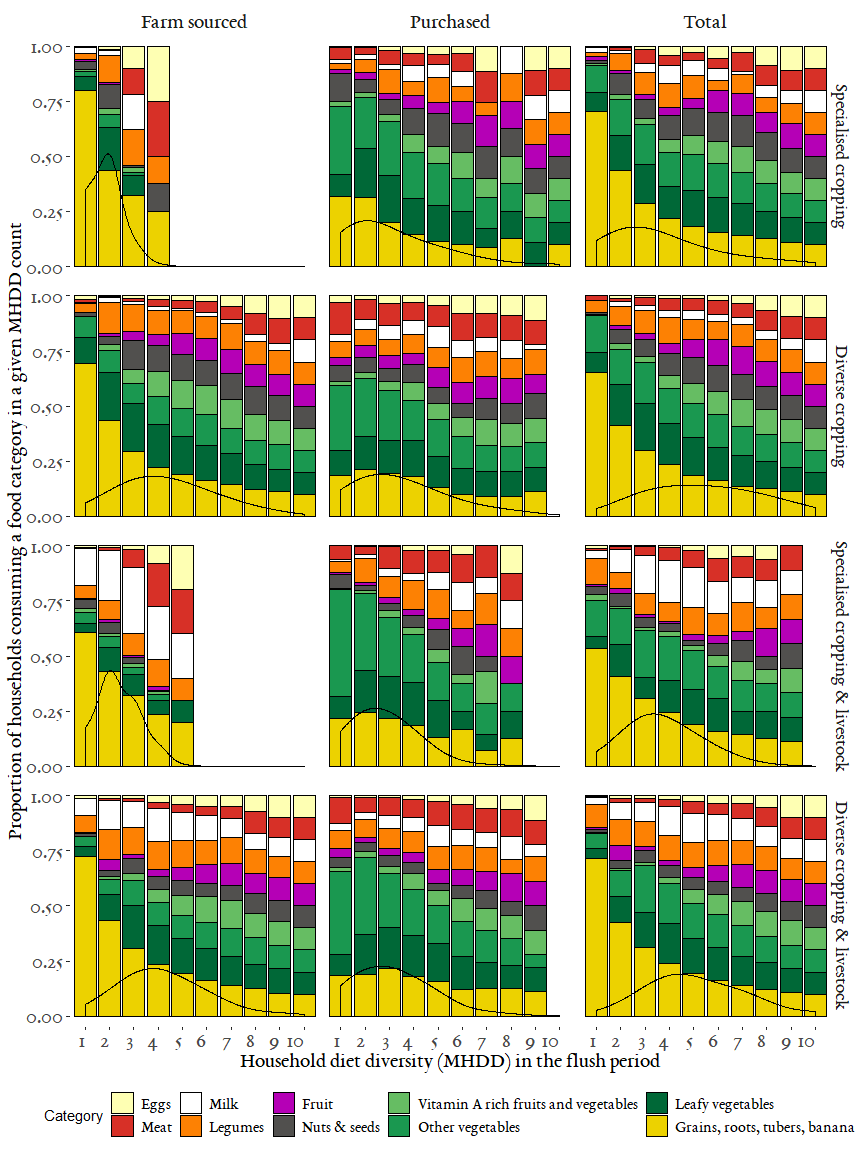
\includegraphics[width=1\textwidth]{Appendix/Ch6_4.png}
    \captionsetup{singlelinecheck = false, justification=justified} %left justify caption
  \caption{Diet diversity: density and proportion of households (n = 6,353) consuming specific food categories by farm type and channel of access in the flush period. The distribution (probability density function) of diet diversity for each period is represented as a black line on the lower half of each figure facet. Food categories are represented by different colours, showing the proportion of households consuming each category at specific diet diversity levels}
  \label{fig:A_4}
\end{figure}

\begin{figure}[H]
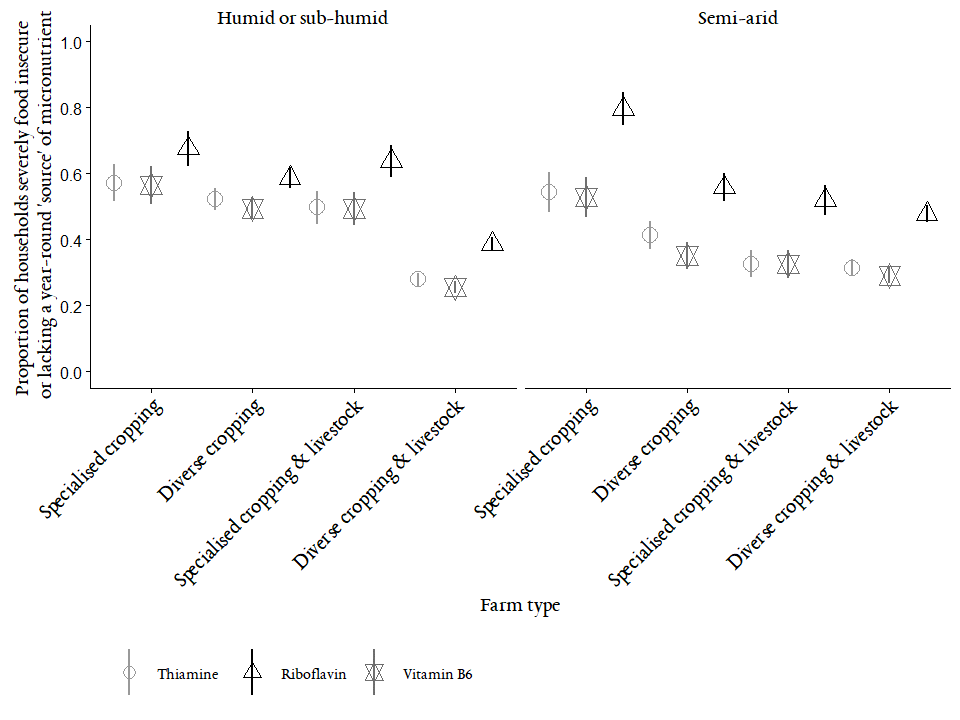
\includegraphics[width=1\textwidth]{Appendix/Ch6_prevalenceOther.png}
    \captionsetup{singlelinecheck = false, justification=justified} %left justify caption
  \caption{Proportion of households (n = 6,353) weighted by population with insecure access to food (MHFIAP) or no `source' of thiamine, riboflavin or vitamin B6 by farm type and agroecological zone. A 95\% confidence interval is represented by vertical lines}
  \label{fig:A_5}
\end{figure}

\begin{itemize}
\item The difference in severe food insecurity prevalence is minimal.

\item Micronutrient estimates are consistently lower for `cropping' households when the threshold is set to 0.5 TLU. The statistically significant difference between `cropping' and `livestock' households, however, remains.

\item A threshold based on animal protein produced was also considered, but is not as suited for a farm type categorisation because it is not as easily observed as TLUs.

\end{itemize}


\begin{table}[H]
  \captionsetup{singlelinecheck = false, justification=justified}
  \caption{Questions asked in MHFIAP and FIES}
  \label{tab:C_10}
  \small
\begin{tabularx}{\textwidth}{
p{\dimexpr 0.37\linewidth-2\tabcolsep}
p{\dimexpr 0.04\linewidth-2\tabcolsep}
p{\dimexpr 0.59\linewidth-2\tabcolsep}}
\toprule
MHFIAP & & FIES \\
\midrule
Did you worry that your household would not have enough food? & & Was there a time when you were worried you would not have enough food to eat because of a lack of money or other resources \\
 & & \\
Was anyone unable to eat your preferred foods due to lack of resources? & & Was there a time when you were unable to eat healthy and nutritious food because of a lack of money or other resources? \\
 & & \\
Did anyone have to eat a limited variety of foods due to lack of resources? & & Was there a time when you ate only a few kinds of foods because of a lack of money or other resources? \\
 & & \\
Did anyone have to eat undesirable foods due to lack of resources? & & Was there a time when you had to skip a meal because there was not enough money or other resources to get food? \\
 & & \\
Did anyone have to eat smaller meals than was felt needed because of limitations in food availability? & & Was there a time when you ate less than you thought you should because of a lack of money or other resources? \\
 & & \\
Did anyone have to eat fewer meals in a day due to a lack of food? & & \\
 & & \\
Was there ever no food of any kind in your household because of a lack of resources? & & Was there a time when your household ran out of food because of a lack of money or other resources? \\
 & & \\
Did anyone go to sleep at night hungry because there was not enough food? & & Was there a time when you were hungry but did not eat because there was not enough money or other resources for food? \\
 & & \\
Did anyone go a whole day and night without eating because there was not enough food? & & Was there a time when you went without eating for a whole day because of a lack of money or other resources? \\
\bottomrule
\end{tabularx}
\end{table}


\begin{table}[H]
  \captionsetup{singlelinecheck = false, justification=justified}
  \caption{Prevalence estimates derived from Martin-Pr\'{e}vel et al. (2015)}
  \label{tab:C_11}
  \small
\begin{tabularx}{\textwidth}{@{}lYYYYYYYY@{}}
%  {
%p{\dimexpr 0.29\linewidth-2\tabcolsep}
%p{\dimexpr 0.09\linewidth-2\tabcolsep}
%p{\dimexpr 0.09\linewidth-2\tabcolsep}
%p{\dimexpr 0.09\linewidth-2\tabcolsep}
%p{\dimexpr 0.09\linewidth-2\tabcolsep}
%p{\dimexpr 0.1\linewidth-2\tabcolsep}
%p{\dimexpr 0.09\linewidth-2\tabcolsep}
%p{\dimexpr 0.09\linewidth-2\tabcolsep}
%p{\dimexpr 0.09\linewidth-2\tabcolsep}}
\toprule
 & & \multicolumn{7}{l}{Probability of adequacy (mean)} \\
 & n & Ca & Fe & Thiamine & Riboflavin & Niacin & Vitamin B6 & Vitamin B12 \\
 \midrule
Burkina Faso 1 & 182 & 0.03 & 0.23 & 0.39 & 0.08 & 0.17 & 0.53 & 0.07 \\
Burkina Faso 2 & 407 & 0.23 & 0.51 & 0.43 & 0.47 & 0.71 & 0.36 & 0.03 \\
Mali & 102 & 0.04 & 0.53 & 0.6 & 0.28 & 0.31 & 0.67 & 0.17 \\
Uganda 1 & 452 & 0.06 & 0.08 & 0.84 & 0.33 & 0.76 & 0.97 & 0.18 \\
Uganda 2 & 954 & 0.07 & 0.13 & 0.77 & 0.56 & 0.73 & 0.83 & 0.03 \\
Total & 2097 & 197 & 464 & 1422 & 918 & 1392 & 1542 & 152 \\
Weighted probability adequate & & 0.09 & 0.22 & 0.68 & 0.44 & 0.66 & 0.74 & 0.07 \\
Weighted deficiency prevalence & & 0.91 & 0.78 & 0.32 & 0.56 & 0.34 & 0.26 & 0.93 \\
\bottomrule
\end{tabularx}
\end{table}


\vspace{1cm}

\begin{table}[H]
  \captionsetup{singlelinecheck = false, justification=justified}
  \caption{
  Association between farm-household-diet characteristics and farm type -- non-livestock oriented vs. livestock orientated. Mixed-effects regressions.
  }
  \label{tab:C_12}
  \small
\begin{tabular}{L{5cm} C{2.5cm} C{2.5cm} C{2cm} C{2cm}}
\toprule
Dependent variable & Intercept estimate (SE) & $\hat{\beta}$\textsubscript{livestock} estimate (SE)$^{\dag}$ &  \\
\midrule
Household inhabitants (Adult eq) & 5.46 (0.51) & 0.92 (0.13) & * \\
Land cultivated (ha) & 1.95 (0.49) & 0.72 (0.20) & * \\
Livestock holdings (TLU) & 3.18 (4.08) & 8.64 (1.16) & * \\
Progress out of poverty & 33.68 (6.73) & 3.45 (0.56) & * \\
MHDDS flush period$^{\ddag}$ & 1.86 (0.08) & 0.04 (0.02) & * \\
MHDDS lean period$^{\ddag}$ & 1.44 (0.10) & 0.12 (0.02) & * \\
Milk consumed in lean period$^\psi$ & -1.33 (0.71) & 1.39 (0.11) & * \\
Meat consumed in lean period$^\psi$ & -0.80 (0.46) & 0.45 (0.11) & * \\
Eggs consumed in lean period$^\psi$ & -2.08 (0.39) & 0.63 (0.11) & * \\
\bottomrule
\end{tabular}
\footnotesize
\raggedright
%\caption*{
\\
95\% CI does not cross zero \\
$^{\dag}$Reference category is `non-livestock oriented farm types' \\
$^{\ddag}$Negative binomial regression \\
$^\psi$Logistic regression. Reference category is `did not consume'
\end{table}


\begin{table}[H]
  \captionsetup{singlelinecheck = false, justification=justified}
  \caption{
  Association between farm-household-diet characteristics and farm type -- specialised cropping vs. diverse. Mixed-effects linear regressions.
  }
  \label{tab:C_12}
  \small
\begin{tabular}{L{5cm} C{2.5cm} C{2.5cm} C{2cm} C{2cm}}
\toprule
Dependent variable & Intercept estimate (SE) & $\hat{\beta}$\textsubscript{diverse} estimate (SE)$^{\dag}$ &  \\
\midrule
Market participation (proportion kcal sold) & 0.25 (0.05) & 0.07 (0.01) & * \\
Crop income (PPP) & 8.74 (21.30) & 0.49 (7.63) & \\
Vitamin A rich consumed in lean period$^\psi$ & 0.31 (0.41) & 0.51 (0.08) & * \\
Dark leafy veg consumed in lean period$^\psi$ & 2.27 (0.58) & 1.02 (0.11) & * \\
Other veg consumed in lean period$^\psi$ & 2.50 (0.53) & 0.51 (0.11) & * \\
Fruit consumed in lean period$^\psi$ & -0.32 (0.59) & 0.52 (0.08) & * \\
Nuts/seeds consumed in lean period$^\psi$ & -0.34 (0.08) & 0.50 (0.08) & * \\
\bottomrule
\end{tabular}
\footnotesize
\raggedright
%\caption*{
\\
95\% CI does not cross zero \\
$^{\dag}$Reference category is `non-livestock oriented farm types'
\end{table}




\begin{table}[H]
  \captionsetup{singlelinecheck = false, justification=justified}
  \caption{
  Association between severe food insecurity / micronutrient access and diverse cropping, livestock keeping households in humid \& sub-humid zones. Mixed-effects logistic regressions.
  }
  \label{tab:C_13_2}
  \small
\begin{tabular}{L{5cm} C{2.5cm} C{2.5cm} C{2cm} C{2cm}}
\toprule
Dependent variable & Intercept estimate (SE) & $\hat{\beta}$\textsubscript{diverse \& livestock} estimate (SE)$^{\dag}$ &  \\
\midrule
Severely food insecure$^{\ddag}$ & -0.86 (0.73) & -0.15 (0.16) & * \\
Calcium$^{\ddag}$ & -2.27 (0.99) & 0.98 (0.16) & * \\
Iron$^{\ddag}$ & -0.05 (0.37) & 0.67 (0.13) & * \\
Thiamine$^{\ddag}$ & 0.01 (0.32) & 0.67 (0.13) & * \\
Riboflavin$^{\ddag}$ & -0.27 (0.37) & 0.52 (0.19) & * \\
Niacin$^{\ddag}$ & -0.27 (0.48) & 0.63 (0.15) & * \\
Pyridoxine$^{\ddag}$ & 0.16 (0.39) & 0.61 (0.13) & * \\
Cobalamin$^{\ddag}$ & -1.58 (0.57) & 0.85 (0.15) & * \\
\bottomrule
\end{tabular}
\footnotesize
\raggedright
%\caption*{
\\
95\% CI does not cross zero \\
$^{\dag}$Reference category is `specialised or no livestock component' \\
$^{\ddag}$Reference category is `did not consume'
\end{table}

\begin{table}[H]
  \captionsetup{singlelinecheck = false, justification=justified}
  \caption{
  Association between severe food insecurity / micronutrient access and specialised cropping, livestock keeping farm types in arid semi-arid zones. Mixed-effects logistic regressions.
  }
  \label{tab:C_13_3}
  \small
\begin{tabular}{L{5cm} C{2.5cm} C{2.5cm} C{2cm} C{2cm}}
\toprule
Dependent variable & Intercept estimate (SE) & $\hat{\beta}$\textsubscript{livestock} estimate (SE)$^{\dag}$ &  \\
\midrule
Chronic hunger$^{\ddag}$ & 0.34 (0.71) & 0.64 (0.14) & * \\
Calcium$^{\ddag}$ & -1.96 (1.27) & 0.99 (0.19) & *\\
Iron$^{\ddag}$ & 0.87 (0.92) & 0.17 (0.15) &  \\
Thiamine$^{\ddag}$ & 0.83 (0.81) & 0.18 (0.15) &  \\
Riboflavin$^{\ddag}$ & -0.24 (1.25) & 0.23 (0.17) &  \\
Niacin$^{\ddag}$ & 0.64 (0.92) & 0.27 (0.59) &  \\
Pyridoxine$^{\ddag}$ & 1.17 (1.03) & 0.08 (0.16) &  \\
Cobalamin$^{\ddag}$ & -2.01 (1.27) & 1.23 (0.18) & * \\
\bottomrule
\end{tabular}
\footnotesize
\raggedright
%\caption*{
\\
95\% CI does not cross zero \\
$^{\dag}$Reference category is `no livestock component' \\
$^{\ddag}$Reference category is `did not consume'
\end{table}



\begin{table}[H]
  \captionsetup{singlelinecheck = false, justification=justified}
  \caption{
  Association between farm-household-diet characteristics and the presence of children. Mixed-effects regressions.
  }
  \label{tab:C_14}
  \small
\begin{tabular}{L{5cm} C{2.5cm} C{2.5cm} C{2cm} C{2cm}}
\toprule
Dependent variable & Intercept estimate (SE) & $\hat{\beta}$\textsubscript{children} estimate (SE)$^{\dag}$ &  \\
\midrule
Household inhabitants (Adult eq) & 4.38 (0.45) & 2.21 (0.11) & * \\
Age of household head & 66.39 (11.33) & -3.45 (4.15) & \\
Land cultivated (ha) & 2.09 (0.49) & 0.42 (0.17) & * \\
Livestock holdings (TLU) & 4.48 (4.85) & 4.85 (0.99) & * \\
Gross income (PPP) & 1479.95 (411.92) & 0.60 (8.73) &  \\
Progress out of poverty & 43.00 (7.46) & -9.61 (0.46) & * \\
\bottomrule
\end{tabular}
\footnotesize
\raggedright
%\caption*{
\\
95\% CI does not cross zero \\
$^{\dag}$Reference category is `no children' \\
$^{\ddag}$Negative binomial regression
\end{table}


\begin{table}[H]
  \captionsetup{singlelinecheck = false, justification=justified}
  \caption{
  Association between chronic hunger (severe food insecurity) and micronutrient access and scale for diverse cultivating, livestock keeping farm types in humid \& sub-humid zones. Mixed-effects logistic regressions.
  }
  \label{tab:C_15}
  \small
\begin{tabular}{L{5cm} C{2.5cm} C{2.5cm} C{2cm} C{2cm}}
\toprule
Dependent variable & Intercept estimate (SE) & $\hat{\beta}$\textsubscript{medium-large} estimate (SE)$^{\dag}$ &  \\
\midrule
Chronic hunger$^{\ddag}$ & -0.37 (0.32) & -0.70 (0.20) & * \\
Calcium$^{\ddag}$ & -1.57 (1.21) & 0.42 (0.26) & * \\
Iron$^{\ddag}$ & 0.38 (0.74) & 0.25 (0.24) & \\
Thiamine$^{\ddag}$ & 0.49 (0.64) & 0.28 (0.23) & \\
Riboflavin$^{\ddag}$ & 0.07 (0.60) & -0.04 (0.20) &  \\
Niacin$^{\ddag}$ & -0.05 (0.84) & 0.62 (0.27) & * \\
Pyridoxine$^{\ddag}$ & 0.53 (0.75) & 0.41 (0.22) &  \\
Cobalamin$^{\ddag}$ & -1.05 (0.98) & 0.45 (0.24) &  \\
\bottomrule
\end{tabular}
\footnotesize
\raggedright
%\caption*{
\\
95\% CI does not cross zero \\
$^{\dag}$Reference category is `small scale' \\
$^{\ddag}$Reference category is `did not consume'
\end{table}


\begin{table}[H]
  \captionsetup{singlelinecheck = false, justification=justified}
  \caption{
  Association between chronic hunger (severe food insecurity) and micronutrient access and scale for specialised cropping, livestock keeping farm types in arid semi-arid zones. Mixed-effects logistic regressions.
  }
  \label{tab:C_16}
  \small
\begin{tabular}{L{5cm} C{2.5cm} C{2.5cm} C{2cm} C{2cm}}
\toprule
Dependent variable & Intercept estimate (SE) & $\hat{\beta}$\textsubscript{medium-large} estimate (SE)$^{\dag}$ &  \\
\midrule
Chronic hunger$^{\ddag}$ & -0.84 (5.93) & 0.45 (0.22) & * \\
Calcium$^{\ddag}$ & -1.99 (1.91) & 0.30 (0.30) & \\
Iron$^{\ddag}$ & 1.04 (1.01) & 0.50 (0.26) & * \\
Thiamine$^{\ddag}$ & 1.04 (1.00) & 0.49 (0.27) & * \\
Riboflavin$^{\ddag}$ & -0.56 (1.54) & 0.44 (0.28) &  \\
Niacin$^{\ddag}$ & 0.97 (1.08) & 0.30 (0.27) &  \\
Pyridoxine$^{\ddag}$ & 1.08 (0.93) & 0.55 (0.27) & * \\
Cobalamin$^{\ddag}$ & -1.57 (2.02) & -0.11 (0.31) & \\
\bottomrule
\end{tabular}
\footnotesize
\raggedright
%\caption*{
\\
95\% CI does not cross zero \\
$^{\dag}$Reference category is `small scale' \\
$^{\ddag}$Reference category is `did not consume'
\end{table}
